\chapter{Auswertung}\label{cha:auswertung}
\section{Ausgehobene Daten}\label{sec:aushebungDaten}
Dieses Kapitel soll zeigen wie genau das Ergebnis für eine Elementarladung wurde. Für das muss aber zuerst ein Blick auf die Daten gemacht werden, die herausgekommen sind beim Experimentieren. In der \autoref{tab:ergebnisse} befinden sich die Spalten, Steig und Fallgeschwindigkeit, Radius, Masse und Ladung des Tröpfchens. 

\begin{table}[h]
	\centering
	\begin{tabular}{llllll}
		\toprule
		Nr. & $v_{rise}$ & $v_{fall}$ & Radius & Masse & Ladung \\
		\midrule
		1 &$\mathrm{2.01 \cdot 10^{-04}}$ & $\mathrm{2.12 \cdot 10^{-05}}$ & $\mathrm{4.04 \cdot 10^{-07}}$ & $\mathrm{2.45 \cdot 10^{-16}}$ & $\mathrm{3.27 \cdot 10^{-19}}$ \\
		2 &$\mathrm{8.46 \cdot 10^{-05}}$ & $\mathrm{2.16 \cdot 10^{-05}}$ & $\mathrm{4.08 \cdot 10^{-07}}$ & $\mathrm{2.53 \cdot 10^{-16}}$ & $\mathrm{1.59 \cdot 10^{-19}}$ \\
		3 &$\mathrm{8.68 \cdot 10^{-05}}$ & $\mathrm{1.98 \cdot 10^{-05}}$ & $\mathrm{3.90 \cdot 10^{-07}}$ & $\mathrm{2.20 \cdot 10^{-16}}$ & $\mathrm{1.51 \cdot 10^{-19}}$ \\
		4 &$\mathrm{8.91 \cdot 10^{-05}}$ & $\mathrm{2.04 \cdot 10^{-05}}$ & $\mathrm{3.96 \cdot 10^{-07}}$ & $\mathrm{2.31 \cdot 10^{-16}}$ & $\mathrm{1.58 \cdot 10^{-19}}$ \\
		5 &$\mathrm{1.97 \cdot 10^{-04}}$ & $\mathrm{1.98 \cdot 10^{-05}}$ & $\mathrm{3.89 \cdot 10^{-07}}$ & $\mathrm{2.18 \cdot 10^{-16}}$ & $\mathrm{3.05 \cdot 10^{-19}}$ \\
		6 &$\mathrm{1.98 \cdot 10^{-04}}$ & $\mathrm{2.04 \cdot 10^{-05}}$ & $\mathrm{3.96 \cdot 10^{-07}}$ & $\mathrm{2.31 \cdot 10^{-16}}$ & $\mathrm{3.14 \cdot 10^{-19}}$ \\
		7 &$\mathrm{9.33 \cdot 10^{-05}}$ & $\mathrm{1.84 \cdot 10^{-05}}$ & $\mathrm{3.74 \cdot 10^{-07}}$ & $\mathrm{1.95 \cdot 10^{-16}}$ & $\mathrm{1.50 \cdot 10^{-19}}$ \\
		8 &$\mathrm{1.26 \cdot 10^{-04}}$ & $\mathrm{1.71 \cdot 10^{-05}}$ & $\mathrm{3.61 \cdot 10^{-07}}$ & $\mathrm{1.74 \cdot 10^{-16}}$ & $\mathrm{1.85 \cdot 10^{-19}}$ \\
		9 &$\mathrm{1.12 \cdot 10^{-04}}$ & $\mathrm{1.23 \cdot 10^{-05}}$ & $\mathrm{3.01 \cdot 10^{-07}}$ & $\mathrm{1.01 \cdot 10^{-16}}$ & $\mathrm{1.29 \cdot 10^{-19}}$ \\
		10 &$\mathrm{1.30 \cdot 10^{-04}}$ & $\mathrm{1.29 \cdot 10^{-05}}$ & $\mathrm{3.08 \cdot 10^{-07}}$ & $\mathrm{1.09 \cdot 10^{-16}}$ & $\mathrm{1.53 \cdot 10^{-19}}$ \\
		11 &$\mathrm{1.26 \cdot 10^{-04}}$ & $\mathrm{1.15 \cdot 10^{-05}}$ & $\mathrm{2.89 \cdot 10^{-07}}$ & $\mathrm{8.97 \cdot 10^{-17}}$ & $\mathrm{1.37 \cdot 10^{-19}}$ \\
		12 &$\mathrm{1.21 \cdot 10^{-04}}$ & $\mathrm{1.58 \cdot 10^{-05}}$ & $\mathrm{3.45 \cdot 10^{-07}}$ & $\mathrm{1.52 \cdot 10^{-16}}$ & $\mathrm{1.68 \cdot 10^{-19}}$ \\
		13 &$\mathrm{2.26 \cdot 10^{-04}}$ & $\mathrm{1.81 \cdot 10^{-05}}$ & $\mathrm{3.72 \cdot 10^{-07}}$ & $\mathrm{1.91 \cdot 10^{-16}}$ & $\mathrm{3.31 \cdot 10^{-19}}$ \\
		14 &$\mathrm{4.50 \cdot 10^{-04}}$ & $\mathrm{1.21 \cdot 10^{-05}}$ & $\mathrm{2.97 \cdot 10^{-07}}$ & $\mathrm{9.76 \cdot 10^{-17}}$ & $\mathrm{4.79 \cdot 10^{-19}}$ \\
		15 &$\mathrm{2.84 \cdot 10^{-04}}$ & $\mathrm{1.07 \cdot 10^{-05}}$ & $\mathrm{2.76 \cdot 10^{-07}}$ & $\mathrm{7.83 \cdot 10^{-17}}$ & $\mathrm{2.79 \cdot 10^{-19}}$ \\
		16 &$\mathrm{2.43 \cdot 10^{-04}}$ & $\mathrm{1.40 \cdot 10^{-05}}$ & $\mathrm{3.23 \cdot 10^{-07}}$ & $\mathrm{1.25 \cdot 10^{-16}}$ & $\mathrm{2.93 \cdot 10^{-19}}$ \\
		17 &$\mathrm{1.26 \cdot 10^{-04}}$ & $\mathrm{1.28 \cdot 10^{-05}}$ & $\mathrm{3.07 \cdot 10^{-07}}$ & $\mathrm{1.07 \cdot 10^{-16}}$ & $\mathrm{1.48 \cdot 10^{-19}}$ \\
		18 &$\mathrm{3.97 \cdot 10^{-04}}$ & $\mathrm{1.30 \cdot 10^{-05}}$ & $\mathrm{3.10 \cdot 10^{-07}}$ & $\mathrm{1.11 \cdot 10^{-16}}$ & $\mathrm{4.44 \cdot 10^{-19}}$ \\
		19 &$\mathrm{2.49 \cdot 10^{-04}}$ & $\mathrm{1.45 \cdot 10^{-05}}$ & $\mathrm{3.29 \cdot 10^{-07}}$ & $\mathrm{1.32 \cdot 10^{-16}}$ & $\mathrm{3.06 \cdot 10^{-19}}$ \\
		20 &$\mathrm{3.96 \cdot 10^{-05}}$ & $\mathrm{3.36 \cdot 10^{-05}}$ & $\mathrm{5.20 \cdot 10^{-07}}$ & $\mathrm{5.22 \cdot 10^{-16}}$ & $\mathrm{1.46 \cdot 10^{-19}}$ \\
		21 &$\mathrm{1.04 \cdot 10^{-04}}$ & $\mathrm{1.47 \cdot 10^{-05}}$ & $\mathrm{3.31 \cdot 10^{-07}}$ & $\mathrm{1.35 \cdot 10^{-16}}$ & $\mathrm{1.40 \cdot 10^{-19}}$ \\
		22 &$\mathrm{5.22 \cdot 10^{-05}}$ & $\mathrm{2.89 \cdot 10^{-05}}$ & $\mathrm{4.79 \cdot 10^{-07}}$ & $\mathrm{4.08 \cdot 10^{-16}}$ & $\mathrm{1.47 \cdot 10^{-19}}$ \\
		23 &$\mathrm{5.40 \cdot 10^{-05}}$ & $\mathrm{3.06 \cdot 10^{-05}}$ & $\mathrm{4.95 \cdot 10^{-07}}$ & $\mathrm{4.50 \cdot 10^{-16}}$ & $\mathrm{1.59 \cdot 10^{-19}}$ \\
		24 &$\mathrm{5.82 \cdot 10^{-05}}$ & $\mathrm{2.67 \cdot 10^{-05}}$ & $\mathrm{4.59 \cdot 10^{-07}}$ & $\mathrm{3.60 \cdot 10^{-16}}$ & $\mathrm{1.46 \cdot 10^{-19}}$ \\
		25 &$\mathrm{5.34 \cdot 10^{-05}}$ & $\mathrm{2.98 \cdot 10^{-05}}$ & $\mathrm{4.88 \cdot 10^{-07}}$ & $\mathrm{4.30 \cdot 10^{-16}}$ & $\mathrm{1.54 \cdot 10^{-19}}$ \\
		26 &$\mathrm{5.76 \cdot 10^{-05}}$ & $\mathrm{2.79 \cdot 10^{-05}}$ & $\mathrm{4.71 \cdot 10^{-07}}$ & $\mathrm{3.87 \cdot 10^{-16}}$ & $\mathrm{1.52 \cdot 10^{-19}}$ \\
		27 &$\mathrm{5.81 \cdot 10^{-05}}$ & $\mathrm{3.01 \cdot 10^{-05}}$ & $\mathrm{4.91 \cdot 10^{-07}}$ & $\mathrm{4.38 \cdot 10^{-16}}$ & $\mathrm{1.64 \cdot 10^{-19}}$ \\
		28 &$\mathrm{5.32 \cdot 10^{-04}}$ & $\mathrm{1.89 \cdot 10^{-05}}$ & $\mathrm{3.81 \cdot 10^{-07}}$ & $\mathrm{2.06 \cdot 10^{-16}}$ & $\mathrm{7.67 \cdot 10^{-19}}$ \\
		29 &$\mathrm{3.55 \cdot 10^{-04}}$ & $\mathrm{1.90 \cdot 10^{-05}}$ & $\mathrm{3.82 \cdot 10^{-07}}$ & $\mathrm{2.06 \cdot 10^{-16}}$ & $\mathrm{5.21 \cdot 10^{-19}}$ \\
		30 &$\mathrm{3.31 \cdot 10^{-04}}$ & $\mathrm{1.65 \cdot 10^{-05}}$ & $\mathrm{3.54 \cdot 10^{-07}}$ & $\mathrm{1.64 \cdot 10^{-16}}$ & $\mathrm{4.42 \cdot 10^{-19}}$ \\
		31 &$\mathrm{4.85 \cdot 10^{-04}}$ & $\mathrm{1.78 \cdot 10^{-05}}$ & $\mathrm{3.68 \cdot 10^{-07}}$ & $\mathrm{1.85 \cdot 10^{-16}}$ & $\mathrm{6.71 \cdot 10^{-19}}$ \\
		32 &$\mathrm{2.10 \cdot 10^{-04}}$ & $\mathrm{1.66 \cdot 10^{-05}}$ & $\mathrm{3.55 \cdot 10^{-07}}$ & $\mathrm{1.66 \cdot 10^{-16}}$ & $\mathrm{2.89 \cdot 10^{-19}}$ \\
		33 &$\mathrm{1.04 \cdot 10^{-04}}$ & $\mathrm{1.77 \cdot 10^{-05}}$ & $\mathrm{3.67 \cdot 10^{-07}}$ & $\mathrm{1.83 \cdot 10^{-16}}$ & $\mathrm{1.61 \cdot 10^{-19}}$ \\
		34 &$\mathrm{2.14 \cdot 10^{-04}}$ & $\mathrm{7.96 \cdot 10^{-06}}$ & $\mathrm{2.34 \cdot 10^{-07}}$ & $\mathrm{4.75 \cdot 10^{-17}}$ & $\mathrm{1.69 \cdot 10^{-19}}$ \\
		35 &$\mathrm{6.02 \cdot 10^{-04}}$ & $\mathrm{8.06 \cdot 10^{-06}}$ & $\mathrm{2.36 \cdot 10^{-07}}$ & $\mathrm{4.85 \cdot 10^{-17}}$ & $\mathrm{4.70 \cdot 10^{-19}}$ \\
		\bottomrule
	\end{tabular}
	\caption{Ergebnisse der Berechnung}
	\label{tab:ergebnisse}
\end{table}
%\begin{table}
\caption{Ergebnisse der Berechnung}
\label{tab:ergebnisse}
\begin{tabular}{lllll}
\toprule
v_rise & v_fall & Radius & Masse & Ladung \\
\midrule
2.01 \times 10^{-04} & 2.12 \times 10^{-05} & 4.04 \times 10^{-07} & 2.45 \times 10^{-16} & 3.27 \times 10^{-19} \\
8.46 \times 10^{-05} & 2.16 \times 10^{-05} & 4.08 \times 10^{-07} & 2.53 \times 10^{-16} & 1.59 \times 10^{-19} \\
8.68 \times 10^{-05} & 1.98 \times 10^{-05} & 3.90 \times 10^{-07} & 2.20 \times 10^{-16} & 1.51 \times 10^{-19} \\
8.91 \times 10^{-05} & 2.04 \times 10^{-05} & 3.96 \times 10^{-07} & 2.31 \times 10^{-16} & 1.58 \times 10^{-19} \\
1.97 \times 10^{-04} & 1.98 \times 10^{-05} & 3.89 \times 10^{-07} & 2.18 \times 10^{-16} & 3.05 \times 10^{-19} \\
1.98 \times 10^{-04} & 2.04 \times 10^{-05} & 3.96 \times 10^{-07} & 2.31 \times 10^{-16} & 3.14 \times 10^{-19} \\
9.33 \times 10^{-05} & 1.84 \times 10^{-05} & 3.74 \times 10^{-07} & 1.95 \times 10^{-16} & 1.50 \times 10^{-19} \\
1.26 \times 10^{-04} & 1.71 \times 10^{-05} & 3.61 \times 10^{-07} & 1.74 \times 10^{-16} & 1.85 \times 10^{-19} \\
1.12 \times 10^{-04} & 1.23 \times 10^{-05} & 3.01 \times 10^{-07} & 1.01 \times 10^{-16} & 1.29 \times 10^{-19} \\
1.30 \times 10^{-04} & 1.29 \times 10^{-05} & 3.08 \times 10^{-07} & 1.09 \times 10^{-16} & 1.53 \times 10^{-19} \\
1.26 \times 10^{-04} & 1.15 \times 10^{-05} & 2.89 \times 10^{-07} & 8.97 \times 10^{-17} & 1.37 \times 10^{-19} \\
1.21 \times 10^{-04} & 1.58 \times 10^{-05} & 3.45 \times 10^{-07} & 1.52 \times 10^{-16} & 1.68 \times 10^{-19} \\
2.26 \times 10^{-04} & 1.81 \times 10^{-05} & 3.72 \times 10^{-07} & 1.91 \times 10^{-16} & 3.31 \times 10^{-19} \\
4.50 \times 10^{-04} & 1.21 \times 10^{-05} & 2.97 \times 10^{-07} & 9.76 \times 10^{-17} & 4.79 \times 10^{-19} \\
2.84 \times 10^{-04} & 1.07 \times 10^{-05} & 2.76 \times 10^{-07} & 7.83 \times 10^{-17} & 2.79 \times 10^{-19} \\
2.43 \times 10^{-04} & 1.40 \times 10^{-05} & 3.23 \times 10^{-07} & 1.25 \times 10^{-16} & 2.93 \times 10^{-19} \\
1.26 \times 10^{-04} & 1.28 \times 10^{-05} & 3.07 \times 10^{-07} & 1.07 \times 10^{-16} & 1.48 \times 10^{-19} \\
3.97 \times 10^{-04} & 1.30 \times 10^{-05} & 3.10 \times 10^{-07} & 1.11 \times 10^{-16} & 4.44 \times 10^{-19} \\
2.49 \times 10^{-04} & 1.45 \times 10^{-05} & 3.29 \times 10^{-07} & 1.32 \times 10^{-16} & 3.06 \times 10^{-19} \\
3.96 \times 10^{-05} & 3.36 \times 10^{-05} & 5.20 \times 10^{-07} & 5.22 \times 10^{-16} & 1.46 \times 10^{-19} \\
1.04 \times 10^{-04} & 1.47 \times 10^{-05} & 3.31 \times 10^{-07} & 1.35 \times 10^{-16} & 1.40 \times 10^{-19} \\
5.22 \times 10^{-05} & 2.89 \times 10^{-05} & 4.79 \times 10^{-07} & 4.08 \times 10^{-16} & 1.47 \times 10^{-19} \\
5.40 \times 10^{-05} & 3.06 \times 10^{-05} & 4.95 \times 10^{-07} & 4.50 \times 10^{-16} & 1.59 \times 10^{-19} \\
5.82 \times 10^{-05} & 2.67 \times 10^{-05} & 4.59 \times 10^{-07} & 3.60 \times 10^{-16} & 1.46 \times 10^{-19} \\
5.34 \times 10^{-05} & 2.98 \times 10^{-05} & 4.88 \times 10^{-07} & 4.30 \times 10^{-16} & 1.54 \times 10^{-19} \\
5.76 \times 10^{-05} & 2.79 \times 10^{-05} & 4.71 \times 10^{-07} & 3.87 \times 10^{-16} & 1.52 \times 10^{-19} \\
5.81 \times 10^{-05} & 3.01 \times 10^{-05} & 4.91 \times 10^{-07} & 4.38 \times 10^{-16} & 1.64 \times 10^{-19} \\
5.32 \times 10^{-04} & 1.89 \times 10^{-05} & 3.81 \times 10^{-07} & 2.06 \times 10^{-16} & 7.67 \times 10^{-19} \\
3.55 \times 10^{-04} & 1.90 \times 10^{-05} & 3.82 \times 10^{-07} & 2.06 \times 10^{-16} & 5.21 \times 10^{-19} \\
3.31 \times 10^{-04} & 1.65 \times 10^{-05} & 3.54 \times 10^{-07} & 1.64 \times 10^{-16} & 4.42 \times 10^{-19} \\
4.85 \times 10^{-04} & 1.78 \times 10^{-05} & 3.68 \times 10^{-07} & 1.85 \times 10^{-16} & 6.71 \times 10^{-19} \\
2.10 \times 10^{-04} & 1.66 \times 10^{-05} & 3.55 \times 10^{-07} & 1.66 \times 10^{-16} & 2.89 \times 10^{-19} \\
1.04 \times 10^{-04} & 1.77 \times 10^{-05} & 3.67 \times 10^{-07} & 1.83 \times 10^{-16} & 1.61 \times 10^{-19} \\
2.14 \times 10^{-04} & 7.96 \times 10^{-06} & 2.34 \times 10^{-07} & 4.75 \times 10^{-17} & 1.69 \times 10^{-19} \\
6.02 \times 10^{-04} & 8.06 \times 10^{-06} & 2.36 \times 10^{-07} & 4.85 \times 10^{-17} & 4.70 \times 10^{-19} \\
\bottomrule
\end{tabular}
\end{table}


Eine vollständige Messtabelle befindet sich im Anhang. Dort werden auch Messungen aufgeführt, die nicht gut genug waren. Sie wurden bei den Berechnungen nicht berücksichtigt. Diese Daten können jetzt auf ein Punktdiagramm gezeichnet werden. Dabei soll die Y-Achse die Ladung der Tröpfchen sein und die X-Achse die jeweilige Nummerierung. Das Diagramm wurde mit Microsoft Excel erstellt und sieht folgendermassen aus.

\begin{figure}[h]
	\centering
	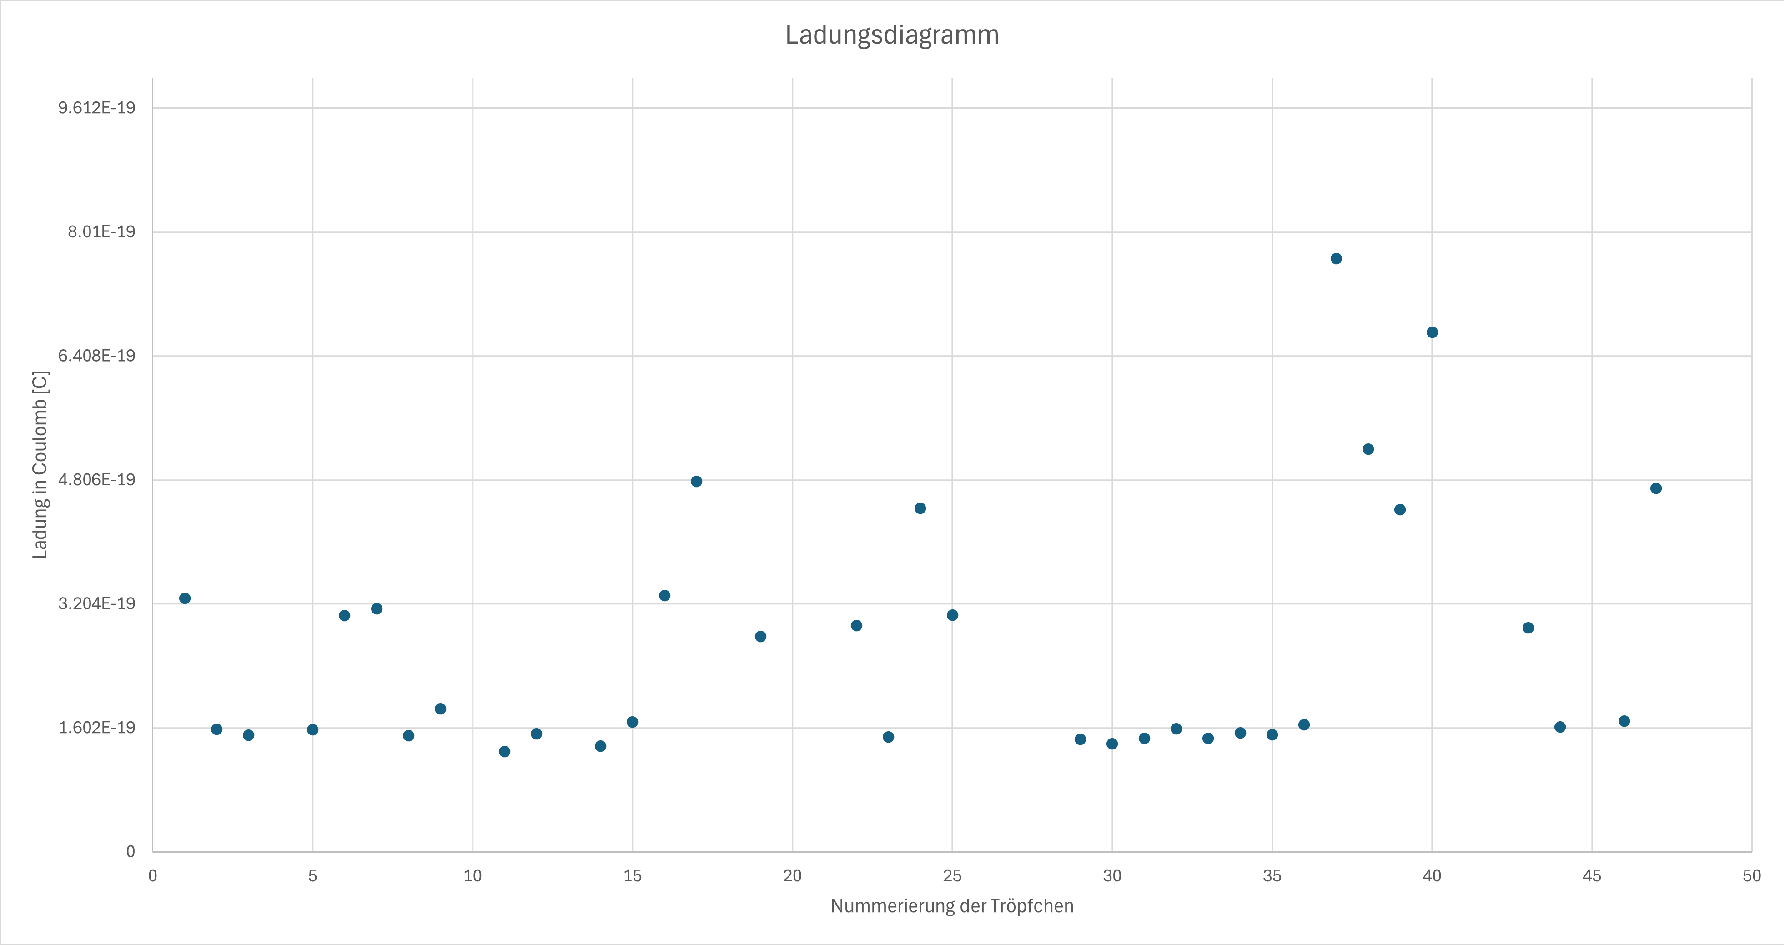
\includegraphics[width=\textwidth]{bilder/pdf/LadungsdiagrammOhne.pdf}
	\caption{Ladungsdiagramm ohne Fehlerrechnung}
	\label{fig:ladungsdiagrammOFehlerrechnung}
\end{figure}

Die Abstände auf der Y-Achse sind nicht zufällig gewählt, sondern ein Linienabstand entspricht exakt einer Elementarladung. Jetzt kann abgelesen werden, wie viele Elementarladungen jedes einzelne Tröpfchen hatte. Es war überraschend zu sehen, wie genau das Experiment geklappt hat. Man sieht, wie sich die Ladungen in Stufen anordnen. Während dem Experimentieren hätte man das nie gedacht. In \autoref{sec:genauigkeitAuswertung} geht man noch auf die Genauigkeit aller Ergebnisse ein, mithilfe einer Fehlerrechnung. Während dem Experimentieren und Auswerten gab es keinen einzigen Sonderfall, der eine viel zu hohe oder tiefe Ladung ergab, das überraschte auch, denn das Experiment hängt von sehr vielen verschiedenen Faktoren und Messgrössen ab.

\section{Das Ergebnis}\label{sec:ergebnis}